\chapter{The Functional Therapeutic Chemical Classification System (Implementation)}

\textbf{Key points}
\begin{itemize}
  \item New mode and mechanism of action (MoA) concepts can be formally created using description logics and following the principles introduced in Chapter 2.
  \item 20,000 new MoA concepts are created and present in a novel resource called the Functional Therapeutic Chemical Classification System (FTC). The resource has a taxonomic structure and describes the biological roles of drugs (e.g. anti-blood coagulation agent).
  \item Over a thousand of approved drugs are classified inside the FTC categories by integrating the content of DrugBank, UniProt and Gene Ontology Annotations (GOA) and with the help of an OWL reasoner. The classification process is fast and complete, as the axioms present in the FTC follow the EL++ profile.
  \item The biomedical information present in the FTC is evaluated against the content of the Anatomical Therapeutic Chemical Classification System (ATC), manually curated resource describing the indication, function and therapeutic areas of approved drugs. Briefly, the drugs classified in the FTC are covering 89\% of the content of the ATC (recall). Given a therapeutic category, the FTC contains more drugs than the ATC, reflecting the drug’s polypharmacology (precision of 50\%).
  \item The content of the FTC will be used to derive systematic drug repositioning hypotheses as presented in Chapter 4.
\end{itemize}

\textbf{Author's comment}

The content and structure of this chapter were directly extracted from the published article \citep{croset2013functional} describing the FTC and some of the analyses performed over it. I have edited the text in order to provide more details when needed and relevant, and to hopefully keep the coherence with the rest of the document. The argumentation has a classical structure: The methodology behind the creation of the resource is first presented, followed by an evaluation section. The results obtained are finally contrasted and discussed.

\hrulefill

\section{Introduction}
Chapter 1 introduced my thesis, namely formally representing drug’s mechanisms and modes of action in order to discover new indications. In Chapter 2 was presented a theoretical perspective on description logics (DLs) and their relation to the study of life. This chapter implements the theory and describes the generation and evaluation of mode of action categories.

As stated in Chapter 1, drug repurposing is the use of known active compounds for new therapeutic indications \citep{sanseau2011editorial}. When administered in a living organism, a compound can indeed play various roles and affect different biological processes; accurately identifying these different functions helps to predict the potential side-effects a drug can have and can also lead to interesting repositioning opportunities \citep{medina2013shifting}. For instance, \emph{sildenafil} was initially developed to relieve angina pectoris symptoms and has been repurposed towards erectile dysfunction during the clinical trials \citep{ashburn2004drug} when a new function of the target enzyme was discovered (see Chapter 1). 

Approved compounds are attractive because they have been extensively studied and have by definition already successfully passed clinical trials, where most drugs fail because of safety or efficacy issues. There is an increasing number of approaches to predict repurposing opportunities using computational methods (see Chapter 1). Most methods operate on the profiles of physicochemical descriptors derived from molecular structures \citep{haupt2011old}. Other methods characterise the drugs on more abstract levels, such as the gene expression signature \citep{iorio2010discovery} or via the reported side-effects \citep{campillos2008drug}. These approaches have in common to look for similarities within existing drugs and forward similar compounds as repurposing hypotheses.

A feature of particular interest to describe drugs is the MoA. According to Wikipedia, the MoA describes \emph{a functional or anatomical change, at the cellular level, resulting from the exposure of a living organism to a substance}. For instance terms such as \emph{transcriptional regulation agent} or \emph{anticoagulant} define MoAs and characterise the roles of a certain type of drug. The MoA abstracts over the relations between molecular functions, protein targets and drug activities; it is the central concept linking a chemical structure to a set of biological activities (see Chapter 1). Intuitively, the indication of a drug logically depends on its MoA (see Figure \ref{fig3-1}).

\begin{figure}[ht]
    \centering
    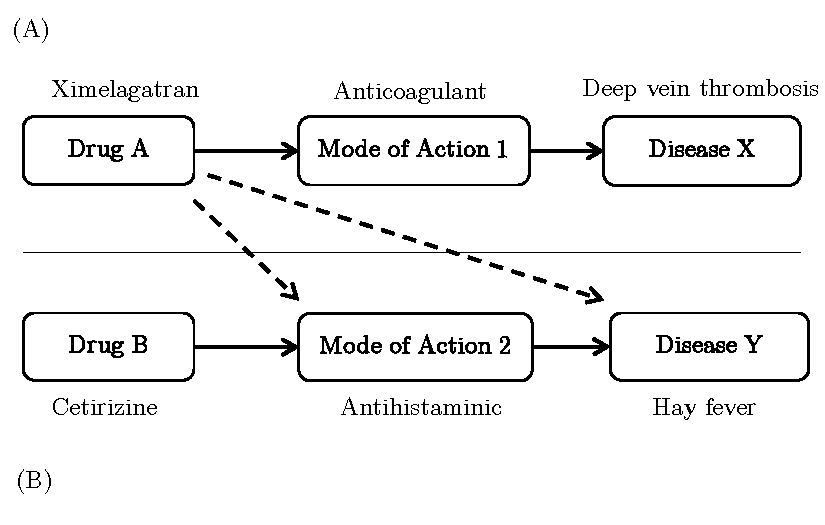
\includegraphics{fig3-1}
    \caption{Conceptual relationship between a drug, its mode of action (MoA) and disease indication. Because a drug exhibits a certain MoA it is therefore indicated for a diseases, as showed by examples (A) and (B). If a new MoA was discovered for a drug (e.g. ximelagatran with antihistaminic MoA), the compound could be re-indicated accordingly (in this case for hay fever – illustrated by the dashed arrows). In order for such a deduction to be made, MoA categories first have to be represented, and secondly drugs have to be assigned to these categories.}
    \label{fig3-1}
\end{figure}

Despite its widespread use in drug discovery, the MoA has not been used yet as a descriptor for repositioning analyses. One reason for this might be the challenge of formally defining the concept. Indeed, MoAs are terms or categories, it is not possible to represent them straightforwardly with values and numbers like one can do for a 3D molecular structure or for a gene expression profile. Nonetheless, the meaning of a concept can be formalised with controlled vocabularies and ontologies \citep{gruber2009encyclopedia}; such frameworks help to formalise the semantics of symbols and strings of characters with explicit axioms (see Chapter 2). 

In an ontology or knowledge base, concepts (interchangeable with \emph{category}, \emph{term} and \emph{class} in this document) are organised and linked following the logical type of relation they have among them. In the Gene Ontology (GO) for example \citep{ashburner2000gene}, biological processes and molecular functions terms are manually curated  and their meaning specified by the relation types linking two GO terms. MoA definitions are present in other classifications such as the Medical Subject Headings \citep{nelson2004mesh} or the Chemical Entities of Biological Interest \citep{hastings2013chebi}. The Anatomical Therapeutic Chemical Classification System (ATC) \citep{world2006anatomical} also describes to some extent the action of drugs at the anatomical level. All these resources are valuable for the community as a source of carefully manually curated information. Moreover, the categories described in these classification systems are sometimes used to annotate drugs: For instance the compound \emph{sildenafil} has been manually annotated as \emph{vasodilator agent} (CHEBI:35620 or MeSH:D27.505.954.411.918).

The classifications mentioned previously are not specially designed for drug repositioning; they purposefully report only the well-known and major MoAs of chemical compounds. The pharmacological spectrum of each drug is not necessarily well covered, yet it would be the best way to predict new indications. In my context, an ideal knowledge base would feature the known MoAs of a drug as well as some predicted ones to be tested in experiments. The MoA categories should derive and scale over primary molecular evidence exposed in biomedical databases, in an automated way as motivated in Chapter 2.

To address the lack of systematic MoA annotations, I have implemented the Functional Therapeutic Chemical Classification System (FTC), presented here in this chapter. The FTC is automatically built by leveraging the content of various biomedical databases using description logics and automated reasoning. Over 20,000 new MoA categories are defined in the resource and further populated with approved drugs using the Web Ontology Language (OWL) in combination with a reasoner. The population step takes in account the type of pharmacological action, the molecular targets of the drugs and their involvement into multiple biological processes.

Drugs can exhibit several MoAs, and the same MoA can be reached through different mechanisms. Most of the drugs are present in multiple FTC categories, reflecting the various roles a compound can play inside a biological system which can serve as starting point for drug repositioning. The resource was evaluated against the ATC, traditional classification scheme introduced before. I present as well some preliminary analyses over the data, by looking at the relation between the MoA and the indication of a compound using semantic similarity. Finer analyses and repositioning use-cases such as Alzheimer’s disease and hypertension will be investigated in Chapter 4.

\section{Method and definitions}
\label{method}

This section describes the building mechanism behind the FTC. The full list of axioms composing the knowledge base are listed at the end of this section (//ref section specification). The FTC is one possible implementation of the theory described in Chapter 2, dedicated to handle MoAs.

Summarised, the creation of the FTC follows these steps: First, a list of categories describing the mode and mechanism of action of drugs is defined. Then in a second step the newly created categories are automatically populated with approved compounds. Finally, the FTC is evaluated and repositioning hypotheses can be generated (presented in Chapter 4).

\subsection{Source code}
The code behind the creation of the resource is entirely open and available at {{https://github.com/loopasam/ftc}}. The web application built on the top of the FTC can be found at {{https://www.ebi.ac.uk/chembl/ftc}} and the documentation can be accessed at {{https://github.com/loopasam/ftc/wiki}}. The reader should be familiar with DLs and the Web Ontology Language (OWL) to fully understand the construction of the knowledge base. An introduction to description logics from the perspective of the biomedical scientist is available on the wiki at {{https://github.com/loopasam/ftc/wiki/Description-Logics}} and in Chapter 2 section. The FTC implementation relies mostly on Brain \citep{croset2013brain} and the web application builds on the top of the Play! framework. Classification tasks use the ELK reasoner \citep{kazakov2013incredible}. The computer hosting the web application has 8 Gb of memory with 4 processors, this architecture allows fast parallel reasoning, thanks to ELK's design. More functionalities will be added to the web application following user requirements (\emph{lean implementation}).

\subsection{Categories creation}
\label{catfunc}

The mode of action categories present in the FTC are defined based on the terms coming from the Gene Ontology (GO). Both the molecular function and biological process branches are used for this purpose, yet handled slightly differently as described below.

\subsubsection{Mode of Action categories}
All the biological processes featured in the GO are looked-up one by one. All the time a process is linked to another process (\emph{X}) via a \emph{positive} or \emph{negative regulation} link, two FTC classes are created: \emph{Anti-X agent} and \emph{Pro-X agent}. For instance the GO term \emph{positive regulation of blood coagulation} is linked to the term \emph{blood coagulation} via a \emph{positively regulates} relation, therefore two FTC categories \emph{Anti-blood coagulation agent} and \emph{Pro-blood coagulation agent} are created. The identifiers of the new FTC classes are also derived from the GO term used to create the class pattern. The GO numeric identifier is re-used and the letter \emph{A} or \emph{P} is appended before to emphasize the \emph{anti} or \emph{pro} pattern. From the example presented previously, the FTC class \emph{Anti-blood coagulation} has FTC\_A0007596 as identifier, because the GO term \emph{blood coagulation} is referenced as GO:0007596. Following the same logic, FTC\_P0007596 is the identifier of the class \emph{Pro-blood coagulation agent}. The design choice for identifiers and labels allows the FTC to fully rely on the high quality work provided by the GO curation team and scale over it.

\subsubsection{Mechanism of Action categories}
The mechanism of actions related to molecular functions are created in the following manner: All the time a molecular function (\emph{Y}) is encountered then two FTC categories are created, as for the processes: \emph{Anti-Y agent} and \emph{Pro-Y agent}. The identifiers are assigned the same way as described before. For instance, out of the GO term \emph{androgen receptor activity} (GO:0004882) two FTC classes are derived: \emph{Pro-androgen receptor activity agent} (FTC\_P0004882) and \emph{Anti-androgen receptor activity agent} (FTC\_A0004882).

\subsection{Equivalent definitions}
FTC classes are generated as presented in the previous section. Up to this point, these categories are only tokens with a human readable label as well as an identifier. The next step is going to assign equivalent definitions to each FTC class. An OWL reasoner can understand such definitions and will automatically classify the knowledge base accordingly, following standard description logics reasoning services (see Chapter 2 section).
Drugs will then be assigned to FTC categories and the taxonomic structure arises after this reasoning step. Equivalent definitions are written as OWL class expressions using the entities of the knowledge base (summarised at {{https://github.com/loopasam/ftc/wiki/Knowledge-Base}} and in section \ref{specs}). There are two types of equivalences: The first one captures perturbation of regulatory biological processes (so called \emph{regulatory patterns}) and the second one handles the perturbed functions (\emph{functional patterns}).

\subsubsection{Regulatory pattern}
Some of the FTC categories are created from the biological processes present in the GO (cf section \ref{catfunc}); these categories have two arbitrary equivalent definitions, representing the two possible ways a compound might impact the biological process. Anti-biological process agent FTC categories contain the drugs that negatively perturb a target involved in the positive regulation of the biological process. The \emph{anti} categories also feature the compounds that positively perturb a negative regulator of the same process. The \emph{pro} categories are equivalent to the opposite pattern. Figure \ref{fig3-2} and \ref{fig3-3} illustrates the equivalent definitions for the FTC classes \emph{Anti-blood coagulation agent} and \emph{Anti-blood coagulation agent}.

\begin{figure}[ht]
    \centering
    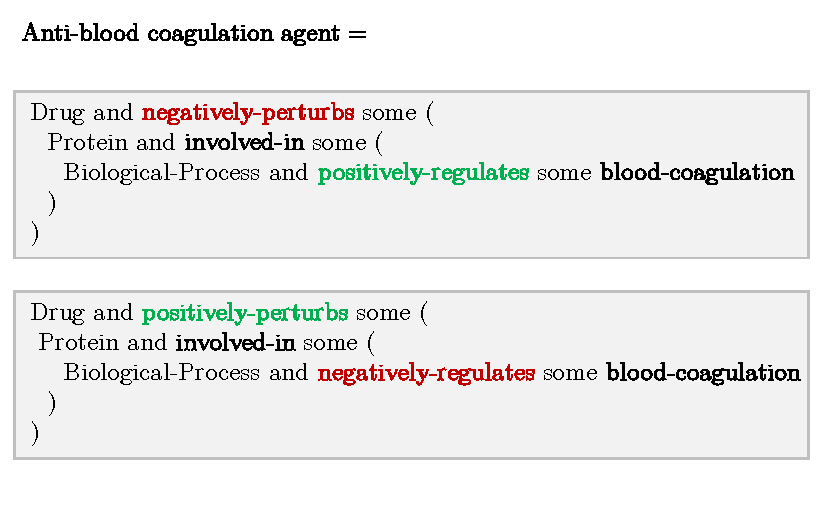
\includegraphics{fig3-2}
    \caption{Regulatory pattern. Equivalent definitions for the concept “Anti-blood coagulation agent”. The concept is asserted as equivalent to either of the boxed expressions. A reasoner can understand such definition and classify drugs accordingly.}
    \label{fig3-2}
\end{figure}

\begin{figure}[H]
    \centering
    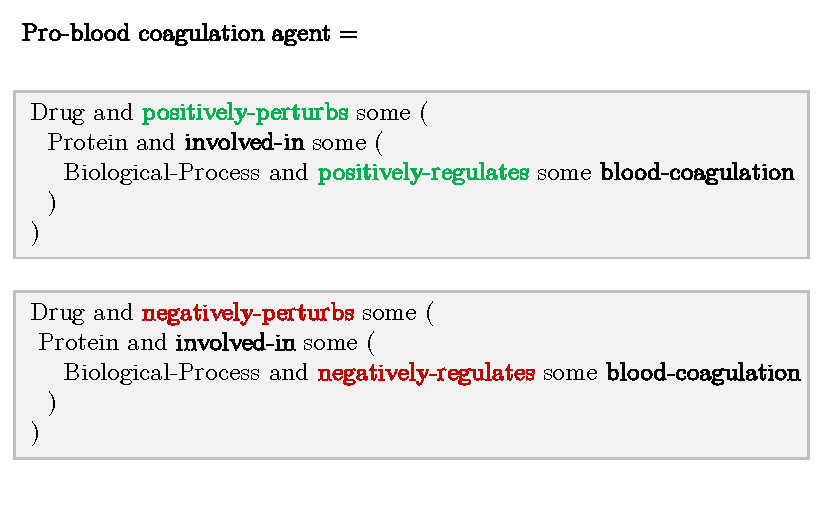
\includegraphics{fig3-3}
    \caption{Example of regulatory pattern. Equivalent definitions for the concept “Pro-blood coagulation agent”. The concept is asserted as equivalent to either of the boxed expressions. A reasoner can understand such definition and classify drugs accordingly.}
    \label{fig3-3}
\end{figure}

Figures \ref{fig3-4} and \ref{fig3-5} present the biological motivation behind the regulatory patterns: it should be easier to adjust the dosage for the compounds classified as such.

\begin{figure}[ht]
    \centering
    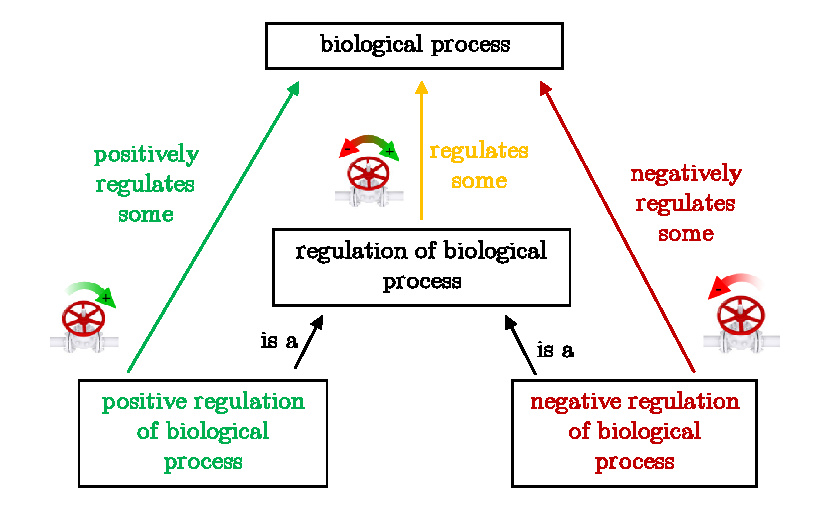
\includegraphics{fig3-4}
    \caption{Biological processes of therapeutic interest are perturbed via regulators of the given process; this strategy allows to modulate and tune the effect, rather than blocking it totally. A regulatory process can be seen as a valve controlling the amplitude or frequency of another process, as defined in the Gene Ontology. This characteristic is of interest for drug discovery, it means that the strength of the pharmacological effect is more likely adaptable with the dosage and drug’s concentration.}
    \label{fig3-4}
\end{figure}

\begin{figure}[H]
    \centering
    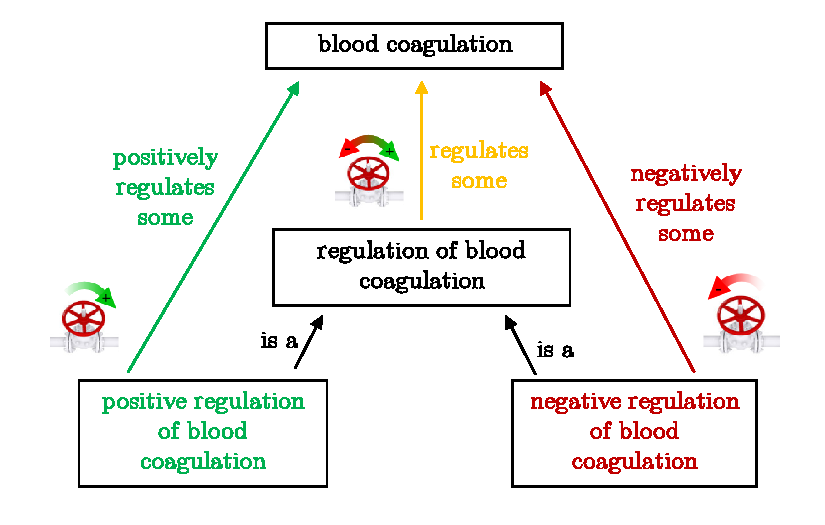
\includegraphics{fig3-5}
    \caption{Example of regulation of the blood coagulation process, as defined in the Gene Ontology. Perturbing the coagulation via a regulator allows to more finely control the therapeutic outcome. See Figure \ref{fig3-4} for theoretical illustration.}
    \label{fig3-5}
\end{figure}

\subsubsection{Functional pattern}
The FTC categories generated from the GO molecular functions (cf section \ref{catfunc}) are also equivalent to a logical definition. \emph{Anti} FTC categories dealing with molecular activities are asserted as equals to the drugs that negatively perturb the function. \emph{Pro} categories are equivalent to the drugs that positively perturb the function of interest. A summary of the functional pattern definitions is available on the online wiki at {{https://github.com/loopasam/ftc/wiki/Mode-of-Action}} and on Figure \ref{fig3-6}.

\begin{figure}[H]
    \centering
    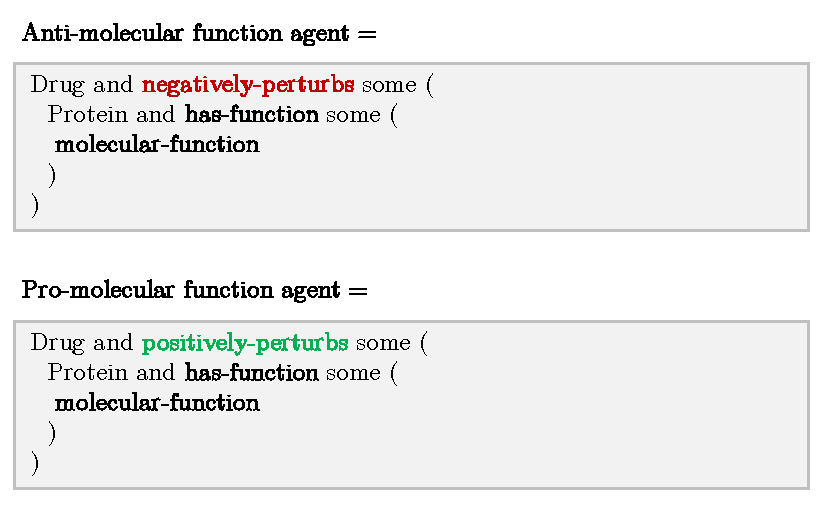
\includegraphics{fig3-6}
    \caption{Example of functional patterns; equivalent definitions for the concepts “pro and anti-molecular function agent”. These concepts is asserted as equivalent to either of the boxed expressions. A reasoner can understand such definition and classify drugs accordingly.}
    \label{fig3-6}
\end{figure}

\subsection{Data integration}
At this stage, the knowledge base contains the created FTC classes associated with their logical definitions, as well as the GO and the core FTC entities. The knowledge base is then further populated with some information coming from various public databases. Only manually curated information extracted from peer-reviewed literature with experimental evidence is considered.

\subsubsection{Drugbank}
The DrugBank database is a unique bioinformatics and cheminformatics resource that combines detailed drug data with comprehensive drug target information \citep{knox2011drugbank}. The approved drugs (small molecules and biotherapeutics) acting on proteins are extracted from the database and imported in the FTC knowledge base. In order to be selected, a compound must firstly be approved and secondly have a pharmacological action on at least one human protein target present in Uniprot \citep{uniprot2013update}. The protein targets all have at least one manually asserted GO annotation \citep{dimmer2012uniprot} for a biological process or a molecular function. DrugBank links compounds to targets via \emph{actions}. The DrugBank actions are somehow structured and consistent: Concepts such as \emph{inhibitor} or \emph{agonist} are reused throughout the database for example, yet they are not strictly formalised as a controlled vocabulary. These actions are manually standardised to the core properties of the FTC according to their biochemical meaning: For instance the action \emph{antagonist} is mapped to the FTC \emph{negatively-perturbs} property. The full list of mappings is available on Table \ref{mappings}.

\begin{center}
\small
    \begin{tabular}{| l | l |}
    \hline
\textbf{DrugBank pharmacological action} & \textbf{mapped FTC property} \\ \hline 
inhibitor & 'negatively-perturbs'\\ \hline 
antagonist & 'negatively-perturbs'\\ \hline 
unknown & 'perturbs'\\ \hline 
agonist & 'positively-perturbs'\\ \hline
potentiator & 'positively-perturbs'\\ \hline 
cofactor & 'perturbs'\\ \hline 
other/unknown & 'perturbs'\\ \hline 
binder & 'perturbs'\\ \hline 
inducer & 'positively-perturbs'\\ \hline 
other & 'perturbs'\\ \hline 
partial agonist & 'positively-perturbs'\\ \hline 
activator & 'positively-perturbs'\\ \hline 
allosteric modulator & 'perturbs'\\ \hline 
negative modulator & 'negatively-perturbs'\\ \hline 
cross-linking/alkylation & 'negatively-perturbs'\\ \hline 
intercalation & 'negatively-perturbs'\\ \hline 
adduct & 'negatively-perturbs'\\ \hline 
chelator & 'negatively-perturbs'\\ \hline 
antibody & 'negatively-perturbs'\\ \hline 
ligand & 'positively-perturbs'\\ \hline 
multitarget & 'perturbs'\\ \hline 
incorporation into and destabilization & 'negatively-perturbs'\\ \hline 
modulator & 'perturbs'\\ \hline 
cleavage & 'negatively-perturbs'\\ \hline 
inverse agonist & 'negatively-perturbs'\\ \hline 
stimulator & 'positively-perturbs'\\ \hline 
suppressor & 'negatively-perturbs'\\ \hline 
partial antagonist & 'perturbs'\\ \hline 
reducer & 'negatively-perturbs'\\ \hline 
inhibitory allosteric modulator & 'negatively-perturbs'\\ \hline 
Binder & 'perturbs'\\ \hline 
inhibitor, competitive & 'negatively-perturbs'\\ \hline 
    \end{tabular} \captionof{table}{Mapping of DrugBank vocabulary to the FTC object properties.}
    \label{mappings}
\end{center}

Compounds coming from DrugBank are represented as OWL classes and asserted as subclasses of the class \emph{DrugBank compound} (FTC\_C2). Protein targets are described as OWL classes too and subclasses of the core class \emph{Protein}. Each DrugBank compound is then connected to its target via the following axiom pattern: \emph{[drug] SubClassOf perturbs some [protein]}. E.g. \emph{Ximelagatran SubClassOf negatively-perturbs some Prothrombin}.

\subsubsection{Gene Ontology Annotations (GOA)}
The GO annotation program aims to provide high-quality GO annotations to proteins in UniProt \citep{dimmer2012uniprot}. In the context of the FTC, such annotations are used to create axioms linking protein targets to molecular functions and biological processes. Each protein annotated with a function creates an axiom such as \emph{[protein] SubClassOf has-function some [molecular function]}. Each protein annotated to a biological process creates an axiom such as \emph{[protein] SubClassOf involved-in some [biological process]}. E.g. \emph{Prothrombin SubClassOf involved-in some positive regulation of blood coagulation}. Each protein can be involved in multiple processes and capable of performing multiple functions; some of the polypharmacology is captured at this level.

\subsection{Knowledge base classification}
The knowledge base is fully built at this step and contains core classes, MoA categories alongside the actions of approved DrugBank compounds on protein targets in Uniprot. The proteins are linked to their molecular functions and involvement in biological processes via the GO annotations. The logical specifications of the FTC are there to glue the different data together and to explicitly express the logical links between resources. The FTC knowledge base follows an OWL2 EL profile \citep{motik2009owl}, which enable the use of fast and parallelised reasoners such as ELK. During the classification process, the reasoner checks whether the MoA equivalent definitions are satisfied or not and assigns drugs inside the corresponding FTC categories. The tree structure of FTC appears also at this step from the logical definitions.

\subsection{Evaluation methodology}
\label{evaluation}

As the classification of therapeutic agents is done in an automated way, it is important to evaluate the results generated against a known resource which will be considered as gold standard. The assessment of the FTC is done against another similar classification, the Anatomical Therapeutic Chemical Classification System (ATC) \citep{world2006anatomical}). The ATC has been developed to serve as a tool for drug utilisation research in order to improve quality of drug use. In this resource, the information is manually curated, and drugs are assigned to categories based of their legally approved indications. Figure \ref{fig3-7} provides a summary of the classification as well as a reference explaining the different levels and their meaning.

\begin{figure}[ht]
    \centering
    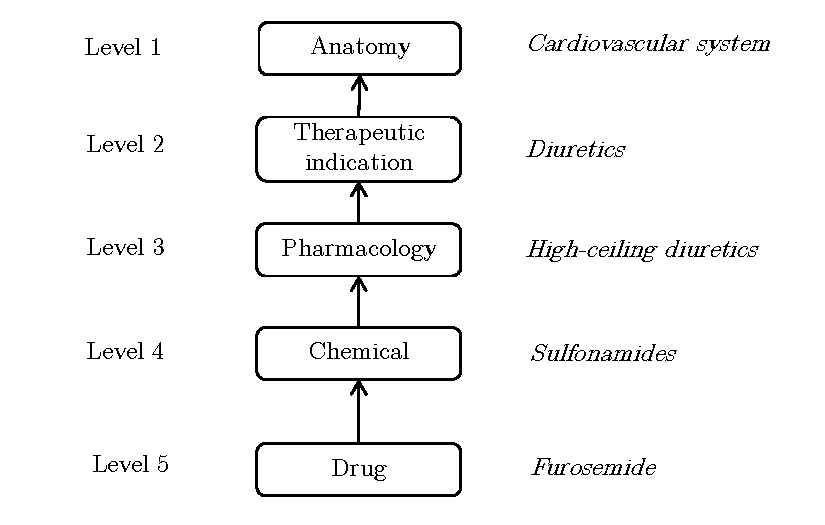
\includegraphics{fig3-7}
    \caption{The structure of the Anatomical Therapeutic Chemical Classification System (ATC). The classification is composed of 5 levels. The first one describes the main anatomical group, the second one reflects the indication or therapeutic area of the drug. Level 3 handles the pharmacological action, level 4 describes the chemical structure, and finally level 5 contains drug’s names. Examples are provided on the right column (italics) for the drug furosemide.}
    \label{fig3-7}
\end{figure}

The goal of the ATC differs from the one of the FTC, yet the two resources are sharing some very similar concepts, which can be used for the evaluation. Categories of both classifications contain approved drugs with a DrugBank identifier, meaning that some of the drugs indexed in the FTC are also present in the ATC. From that, it is possible to define some evaluation points, which will help to assess the automated classification process.

\subsubsection{Evaluation Points}
An evaluation point is defined as an equivalence between a class from the FTC with one or more classes from the ATC. The idea is to look at the set of drugs contained in both side of the equivalence and estimate the overlap, as illustrated in the Figure \ref{fig3-8}.

\begin{figure}[ht]
    \centering
    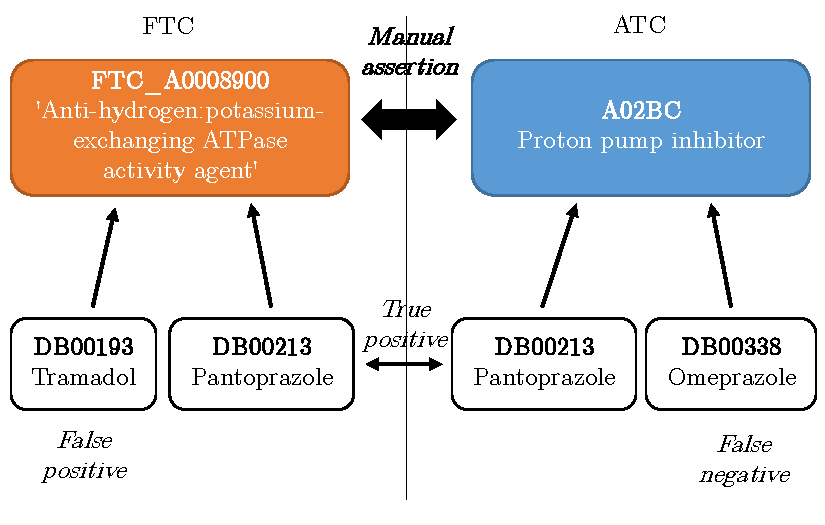
\includegraphics{fig3-8}
    \caption{Example of evaluation point. An manual assertion is made between an ATC category (blue) and a FTC class (orange) when the two concepts are semantically equivalent. Then drugs belonging to each of these classes are compared, and the evaluation can be performed.}
    \label{fig3-8}
\end{figure}

Evaluation points are defined by hand and not themselves evaluated. The full list of evaluation points as well as a summary of the results are available online at https://www.ebi.ac.uk/chembl/ftc/evaluation/. Each evaluation point has a series of true/false positive and false negative drugs associated with it.

\subsubsection{True Positives}
Drugs that are present in both the FTC and the equivalent ATC class(es) are called true positives. These compounds reflect that the automated classification was capable of retrieving correctly the information present in the gold standard (ATC).

\subsubsection{False Negatives}
These drugs are present in the ATC class(es) but not in the corresponding FTC class. The automated classification failed to retrieve these compounds. The smaller the number of false negatives is, the better the FTC is at recalling drugs. A small number of false negatives means that if a drug is present in the ATC (gold standard), then it is likely that the drug will also be correctly categorised in the FTC.

\subsubsection{False Positives}
The false positives are the drugs present in the FTC category of the evaluation point but not in the corresponding ATC classes. A high number of false positives means that the FTC is over-assigning compounds to classes. The false positives relates to the accuracy of the classification. In the context of this work, some false positives could also be considered as drug repurposing opportunities.

\subsubsection{Precision}
Recall is the probability that a randomly selected drug from the ATC has been assigned to the correct corresponding class in the FTC. The value is standardised as a percentage and corresponds to the formula: $ True Positive / (True Positive + False Negative) $.

\subsubsection{Recall}
Recall is the probability that a randomly selected drug from the ATC has been assigned to the correct corresponding class in the FTC. The value is standardised as a percentage and corresponds to the formula: $ True Positive / (True Positive + False Negative) $.

\subsection{Semantic similarity}
The semantic similarity measure performed over the FTC is a derivative of the Jaccard index \citep{jaccard1912distribution} \citep{rogers1960computer} (see Chapter 2 semantic //ref similarity section). It is probably best understood as an example: If two classes A and B are considered, the semantic similarity between these classes corresponds to the number of OWL superclasses (direct and indirect, obtained with a reasoner) that are shared by A and B (intersection) divided by the number of superclasses of A or B (union). The index ranges from 0 (totally different) to 1 (identical). A similar approach was successfully implemented by \citep{hoehndorf2011phenomenet}, for similarity computations over phenotypic traits.

\subsection{Mode of action similarity against indication}
A statistical analysis was performed over the data presented on section (//ref section). When two compounds are randomly taken, they have on average a higher mode of action similarity when they are assigned to the same ATC category (one ATC level). In order to estimate whether this observation was due to chance only, I formulated the following null hypothesis (H0): \emph{For a pair of drug A and B, it does not matter to which ATC category they belong to, their similarity is always average.} The alternative hypothesis (H1) was: \emph{For a pair of drug A and B, if A and B have the same ATC code, I expect on average to obtain a higher similarity value than if A and B have different ATC codes.}

A permutation test was then performed for each ATC category. For example, I started with the ATC category A (first row on Figure //cite), looked at the similarity values when pairs of compounds both belong to the category A (top right corner square) and compared it to the similarity values when the pair of compounds belong to different categories (A and B, A and C and so forth). For each comparison I obtained two distributions of values (not shown). On average the similarity values are always higher when the two compounds belong to the same category (A/A versus A/B for instance). A permutation test (n = 20,000) was performed in order to see whether this observation was due to chance only. I was able to reject the null hypothesis for a significance level of 0.05 all the times. The choice for a permutation test was driven by the fact that MoA similarity values do not follow any type of standard distribution (data not shown).

\subsection{Knowledge base specification}
\label{specskb}

This section presents the scaffold of the knowledge base underlying the FTC. The logic structuring the FTC comes essentially from a set of core OWL properties (rich RBox). Some of these properties originate from the GO. When necessary some new ones have also been introduced. In order to understand how these properties interact, first will be presented the fundamental classes present at the top of the FTC classification, followed by the presentation of the object properties.

\subsubsection{Core FTC classes}

\paragraph{molecular function}
\begin{itemize}
  \item Identifier: http://purl.obolibrary.org/obo/GO\_0003674
  \item Label: 'molecular function'
  \item Definition: As defined by the Gene Ontology: Elemental activities, such as catalysis or binding, describing the actions of a gene product at the molecular level. A given gene product may exhibit one or more molecular functions.
\end{itemize}

\paragraph{biological process}
\begin{itemize}
  \item Identifier: http://purl.obolibrary.org/obo/GO\_0008150
  \item Label: 'biological process'
  \item Definition: As defined by the Gene Ontology: Any process specifically pertinent to the functioning of integrated living units: cells, tissues, organs, and organisms. A process is a collection of molecular events with a defined beginning and end.
\end{itemize}

\paragraph{Protein}
\begin{itemize}
  \item Identifier: http://purl.uniprot.org/core/Protein
  \item Label: 'protein'
  \item Definition: As defined by Uniprot: Description of a protein.
  \item Comment: Gene products present inside the FTC are all human proteins. Uniprot URIs are used.
\end{itemize}

\paragraph{Drug}
\begin{itemize}
  \item Identifier: http://schema.org/Drug
  \item Label: 'drug'
  \item Definition: As defined by schema.org: A chemical or biologic substance, used as a medical therapy, that has a physiological effect on an organism.
  \item Comment: In the context of the FTC, DrugBank chemicals are considered for their role as therapeutic agent rather than for their chemical structure.
\end{itemize}

\paragraph{therapeutic agent}
\begin{itemize}
  \item Identifier: https://www.ebi.ac.uk/chembl/ftc/FTC\_C1
  \item Label: 'therapeutic agent'
  \item Definition: Role of a drug capable of producing a therapeutic effect.
\end{itemize}

\paragraph{DrugBank compound}
\begin{itemize}
  \item Identifier: https://www.ebi.ac.uk/chembl/ftc/FTC\_C2
  \item Label: 'DrugBank compound'
  \item Definition: Drug coming from DrugBank.
\end{itemize}

\subsubsection{Core FTC properties}

\paragraph{part-of}
\begin{itemize}
  \item Identifier: http://purl.obolibrary.org/obo/BFO\_0000050
  \item Characteristic: Transitive
  \item Label: 'part-of'
  \item Definition: As defined and used in the Gene Ontology. More information at http://www.geneontology.org/GO.ontology.relations.shtml\#partof
\end{itemize}

\paragraph{has-part}
\begin{itemize}
  \item Identifier: http://purl.obolibrary.org/obo/BFO\_0000051
  \item Characteristic: Transitive
  \item Label: 'has-part'
  \item Definition: As defined and used in the Gene Ontology. More information at http://www.geneontology.org/GO.ontology-ext.relations.shtml\#haspart
\end{itemize}

\paragraph{regulates}
\begin{itemize}
  \item Identifier: http://purl.obolibrary.org/obo/RO\_0002211
  \item Chained property: 'regulates' o 'part-of' $ \rightarrow $ 'regulates'
  \item Label: 'regulates'
  \item Definition: As defined and used in the Gene Ontology. More information at http://www.geneontology.org/GO.ontology.relations.shtml\#regulates
\end{itemize}

\paragraph{negatively-regulates}
\begin{itemize}
  \item Identifier: http://purl.obolibrary.org/obo/RO\_0002212
  \item SubPropertyOf: 'regulates'
  \item Label: 'negatively-regulates'
  \item Definition: As defined and used in the Gene Ontology. More information at http://www.geneontology.org/GO.ontology.relations.shtml\#regulates
\end{itemize}

\paragraph{positively-regulates}
\begin{itemize}
  \item Identifier: http://purl.obolibrary.org/obo/RO\_0002213
  \item SubPropertyOf: 'regulates'
  \item Label: 'positively-regulates'
  \item Definition: As defined and used in the Gene Ontology. More information at http://www.geneontology.org/GO.ontology.relations.shtml\#regulates
\end{itemize}

\paragraph{involved-in}
\begin{itemize}
  \item Identifier: https://www.ebi.ac.uk/chembl/ftc/FTC\_R1
  \item Label: 'involved-in'
  \item Domain: 'protein'
  \item Range: 'biological process'
  \item Definition: Entails the participation of a protein in a biological process
\end{itemize}

\paragraph{has-function}
\begin{itemize}
  \item Identifier: https://www.ebi.ac.uk/chembl/ftc/FTC\_R2
  \item Label: 'has-function'
  \item Domain: 'protein'
  \item Range: 'molecular function'
  \item Definition: Describes the molecular function born by a protein
\end{itemize}

\paragraph{perturbs}
\begin{itemize}
  \item Identifier: https://www.ebi.ac.uk/chembl/ftc/FTC\_R3
  \item Label: 'perturbs'
  \item Domain: 'drug'
  \item Range: 'protein'
  \item Definition: Specific biochemical interaction through which a drug substance will affect the activity of a protein. The property refers to the specific molecular targets to which the drug binds, such as an enzyme or receptor.
\end{itemize}

\paragraph{negatively-perturbs}
\begin{itemize}
  \item Identifier: https://www.ebi.ac.uk/chembl/ftc/FTC\_R4
  \item Label: 'negatively-perturbs'
  \item SubPropertyOf: 'perturbs'
  \item Definition: Specific biochemical interaction through which a drug substance will decrease the activity of a protein. The property refers to the specific molecular targets to which the drug binds, such as an enzyme or receptor.
\end{itemize}

\paragraph{postively-perturbs}
\begin{itemize}
  \item Identifier: https://www.ebi.ac.uk/chembl/ftc/FTC\_R5
  \item Label: 'postively-perturbs'
  \item SubPropertyOf: 'perturbs'
  \item Definition: Specific biochemical interaction through which a drug substance will increase the activity of a protein. The property refers to the specific molecular targets to which the drug binds, such as an enzyme or receptor.
\end{itemize}

\section{The classification}
The knowledge base behind the FTC is built by integrating information coming from various sources. The GO terms serve as template to create the FTC categories describing the MoAs; DrugBank provides the known links between drugs and their protein targets and Uniprot  maps targets to their respective GO annotations. Drugs are further assigned into MoA categories according to the OWL constructs and axioms defined in the FTC. A reasoner, a program capable of understanding such axioms, performed this task (see the method section \ref{method}). The process to build the FTC is summarised in Figure \ref{fig3-9} alongside an example. 

\begin{figure}[H]
    \centering
    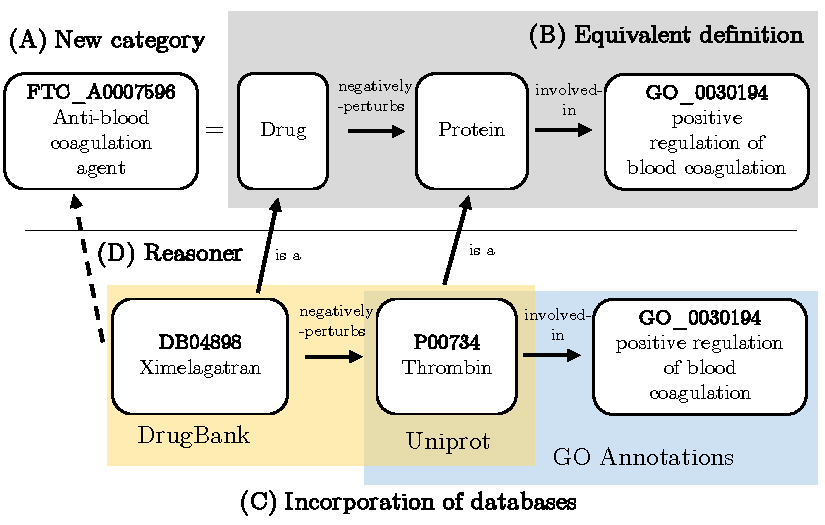
\includegraphics{fig3-9}
    \caption{The diagram gives an overview of the integrated resources and building process. (A) The name of FTC categories representing MoAs are directly derived from the GO terms representing the molecular functions and biological processes. (B) Each of the new FTC class has a logical equivalent definition assigned to it (axiom), representing the necessary and sufficient conditions for a drug to be classified in the corresponding MoA class. (C) The content of various databases is incorporated and linked using the FTC specific logical properties. (D) Finally a reasoner classifies the knowledge base and assigns drugs to MoA classes based on whether or not a definition can be satisfied. For example, the drug \emph{ximelagatran} will be assigned as member of the category \emph{Anti-blood coagulation agent} because of the logical links \emph{ximelagatran negatively-perturbs prothrombin} and \emph{prothrombin involved-in positive regulation of blood coagulation}. The taxonomic structure of the FTC appears also in the reasoning step, from the entailment of the equivalent definitions.}
    \label{fig3-9}
\end{figure}

The core step is the generation of axiomatic representations of MoAs by decomposing GO types into positive and negative regulations of biomolecular functions and processes. The help of reasoning techniques we can further derive and assign MoA across the knowledge base to given drugs. It requires a few seconds (four processing cores, 8 GB RAM) to classify the knowledge base (ELK reasoner). Other OWL reasoners (e.g, Hermit, Pellet, etc.) disqualified mainly due to long processing time (data not shown - see \cite{gonccalves2013owl} for time values).

The FTC forms a taxonomic structure as illustrated on Figure 3-8, which arises when the reasoner classifies the knowledge base. In general, categories may have multiple parents and multiple children (see {{https://www.ebi.ac.uk/chembl/ftc}} for interactive use).

\begin{figure}[ht]
    \centering
    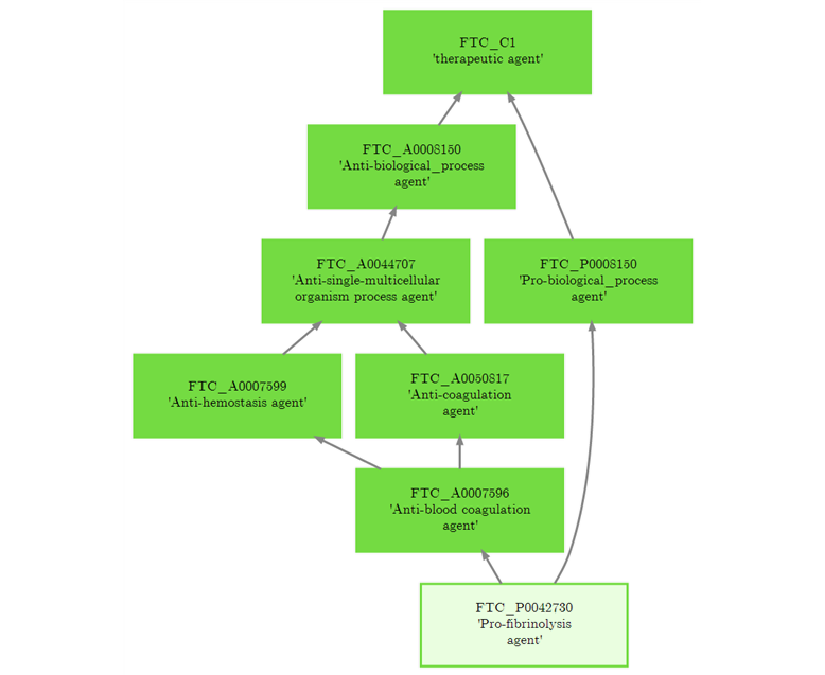
\includegraphics{fig3-10}
    \caption{Parent categories to the FTC class \emph{Pro-fibrinolysis agent} (FTC\_P0042730). The classification is a direct acyclic graph where categories are describing increasingly specific concepts. Arrows entail subclass relationships between the terms (\emph{is a} relation).}
    \label{fig3-10}
\end{figure}

In total there are 1',280 FDA-approved DrugBank compounds (chemical and biotherapeutics) associated with 1'264 human protein targets, where each drug is acting on at least one human protein target. The FTC introduces 23,353 new categories describing the mode and mechanism of action of therapeutic compounds. 4,289 of these categories belong to the biological processes in GO and 19'064 to the molecular functions. A summary of the metrics behind the latest build is available online at {{https://www.ebi.ac.uk/chembl/ftc/evaluation/}}. Out of all FTC categories, 1,432 categories (\textgreater 6\%) directly contain at least one approved drug. This number increases up to 2,532 (\textgreater 11\%) when direct and indirect drugs are considered. FTC categories not containing drugs (e.g, FTC\_A0001771 - \emph{Anti-immunological synapse formation agent}) represent MoAs for which no approved compounds has qualified yet or that have not been identified as such in the FTC.

\section{Evaluation}
The content of the FTC has been evaluated against the drug categorisation of the ATC, which has been produced by manual curation and serves as a gold standard. \emph{A priori}, both resources serve different purposes and as a consequence, the evaluation has to take this into consideration (cf section \ref{interpreting}). The full methodology behind the evaluation is described in the section (section \ref{evaluation}) of the methodology. Briefly, for 68 categories from the FTC one can manually identify a set of semantically equivalent categories in the ATC. I call these equivalent categories the \emph{evaluation points}. All drugs from each evaluation point were then assessed to determine the quality of the FTC against the gold standard, i.e.\ the ATC. For example, the FTC category \emph{Anti-hydrogen:potassium-exchanging ATPase activity agent} (FTC\_A0008900) has been manually asserted as equivalent to the ATC category \emph{Proton pump inhibitors} (A02BC). A summary of this evaluation point is furthermore available online at {{https://www.ebi.ac.uk/chembl/ftc/evaluation/FTC\_A0008900}}.

For 1'280 DrugBank compounds in the FTC, 1,134 are also present in the ATC, therefore only those were considered. The \emph{evaluation points} cover a total of 471 DrugBank compounds or around 41\% of common drugs to both classifications. Out of these, 275 compounds are true positives, i.e.\ they match both, the FTC and ATC categories for a given evaluation point. The \emph{proton pump inhibitor} evaluation point is such a case where all the drugs (\emph{omeprazole, esomeprazole, pantoprazole, lansoprazole, rabeprazole}) are present both in the FTC category and in the corresponding ATC category. The total number of compounds from an ATC category but where it was not possible to identify a corresponding FTC category is 35 (false negatives). Finally, 280 compounds are present in a FTC class but not in any corresponding ATC category (false positives). Overall a recall of 89\% is derived; this percentage indicates that the automatic build of the FTC covers a good portion of the content already present in the ATC. The precision of 50\% shows that the FTC contains for a given MoA many more drugs than the equivalent ATC categories. This result was expected and comes the original idea behind the FTC: Representing in a systematic fashion the implicit and explicit MoAs of drugs, in particular the ones not already indexed by current classification scheme.

\section{Exploration}
The FTC was designed to assist drug repositioning analyses by explicitly representing the polypharmacology of approved drugs. In this section I exemplify how the resource can be used to perform different types of analysis, whose will be extended in Chapter 4.

\subsection{Polypharmacology spectrum}
The more information on a drug’s molecular targets and their physiological roles, the more opportunities exist to re-orient a drug into doing something new. The therapeutic agents described in the FTC can have several MoAs, i.e.\ may be acting on different biomolecular functions or processes, which demonstrates the intrinsic polypharmacology of the approved compounds. 
Figure \ref{fig3-11} illustrates the polypharmacology spectrum by showing the distribution of number of MoAs per compound.

\begin{figure}[H]
    \centering
    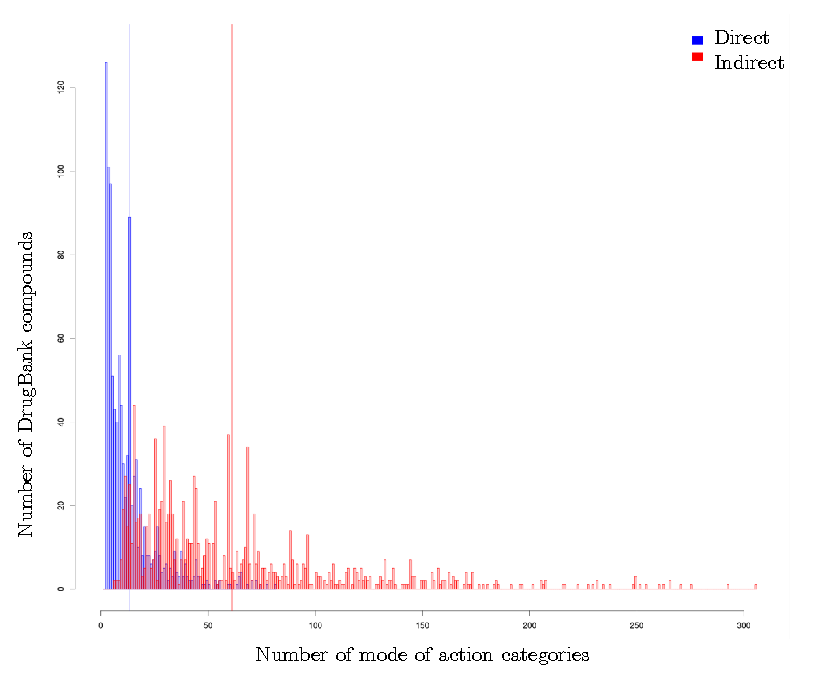
\includegraphics{fig3-11}
    \caption{Distribution of the direct (blue) and indirect (red) number of MoAs per drug. Means are indicated with a solid line. On average each compound has 13.5 MoAs when only direct classes are considered. The number rises
to 61.2 when indirect MoAs are included. Indirect MoAs are the ancestor classes in the taxonomy as shown in Figure XXX. The distribution range is wider when indirect MoAs are considered (range=299; min=7; max=306) versus direct MoAs only (range=79; min=3; max=82). These results emphasises the fact that some drugs are well characterised in databases and could be used for a variety of specific biological tasks. Finally some compounds have been assigned to a small number of FTC categories; in such cases little is known or reported about their pharmacology and repurposing opportunities might be limited.}
    \label{fig3-11}
\end{figure}

When only direct categories are considered, compounds belong on average to 13.5 MoA categories. This number increases to 61.2 when parent categories are taken into consideration (super classes). Not all the MoAs are relevant to a disease, some FTC categories are particularly abstract (e.g, \emph{Anti-biological process agent}) yet they represent discrete categories to which the drug belongs with an explicit and clear meaning. These discrete MoAs are a good starting point to understand what a compound can do when administered in a human system. Compound's polypharmacology is well represented in the FTC, as shown by the numerous MoAs each approved drug can exhibit.

I decided to further look at a well-known repositioning example, in order to see whether the FTC was suitable to identify the new uses of an old drug. I picked \emph{thalidomide} for this exercise ({{https://www.ebi.ac.uk/chembl/ftc/agent/DB01041}}). The molecule was first indicated to treat morning sickness in pregnant women, but has been quickly abandoned after its developmental toxicity has been discovered in newborns (//ref section introduction). The accepted molecular mechanism behind the side-effect is  an impairment of the angiogenic process responsible for the development of members, affecting in particular the limbs \citep{therapontos2009thalidomide}. I found that \emph{thalidomide} was accurately classified as \emph{Anti-cell migration involved in sprouting angiogenesis agent} in the FTC, capturing the known toxicity of the drug. Furthermore, \emph{thalidomide} is currently investigated for a multitude of new usages, in particular for anti-cancer and immunomodulatory activities among others \citep{teo2005thalidomide} and ref chapter 1. These new indications are well represented in the FTC too, for example by the categories \emph{Anti-vascular endothelial growth factor production agent} or \emph{Anti-cell division agent} for antineoplastic activities, or by the classes \emph{Anti-cytokine secretion agent} and \emph{Anti-I-kappaB kinase/NF-kappaB cascade agent} for its effect on the immune system. These observations demonstrate that the FTC can successfully capture the molecular reasons behind the repositioning of an old compound, relying on automated reasoning over integrated electronic evidence. Moreover the classification can also provide valuable insight regarding potential toxicity too.

\subsection{Drugs with similar functions have similar indications}
The list of MoAs attributed to a drug can be exploited as a descriptor for the therapeutic agent: The tree structure of the FTC can be used to derive some similarity metrics over the MoAs. The underlying heuristic is to assume that the closer two entities are in the taxonomy, the more similar they are. We used a straightforward approach derived from the Jaccard index (see method section) in order to compare approved drugs based on the similarity of their MoAs. For instance, the similarity between two compounds present in the same FTC category is 1 (maximum). The similarity between an \emph{anti-blood coagulant} and \emph{pro-blood coagulant} is 0.29, reflecting the fact that such compounds are dissimilar with regards to the outcome of their biological effect. As the MoA is intuitively expected to be the central concept leading to the indication of the drug, we expected that on average, drugs with similar MoAs would be indicated towards similar therapeutic areas.
The heat map presented in Figure \ref{fig3-12} shows a pairwise comparison of all the drugs of the FTC based on their relative MoA similarity.

\begin{figure}[H]
    \centering
    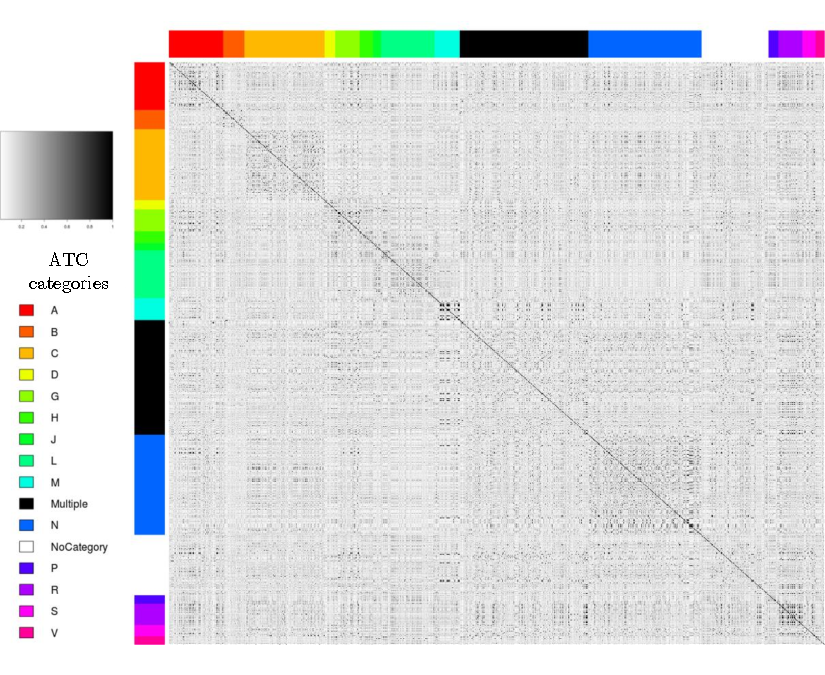
\includegraphics{fig3-12}
    \caption{Pairwise comparison of MoAs similarities. Therapeutic indications are represented by ATC categories which are the colours on the side. For instance, the compound \emph{reteplase} (DB00015) has the ATC code B01AD07, 
which appears as \emph{B} (dark orange) on the plot. Only the first ATC level is considered. The similarity descriptor ranges from 0 (not similar - white) to 1 (identical - black). Some compounds belong to multiple ATC categories (\emph{Multiple}) and some others do not have an ATC code (\emph{NoCategory}). The average similarity of drugs present in the same therapeutic category is significantly higher on average when separately compared to all other indications.}
    \label{fig3-12}
\end{figure}

The compounds are further grouped by therapeutic indications as defined by the ATC. The heatmap reveals some square patches around the central diagonal; the overall similarity appears higher when compounds from the same ATC group are considered. A significance analysis (see method, section XXX) revealed that the average MoA similarity of compounds belonging to the same ATC category is significantly higher than when compounds belonging to different categories are compared. Indeed, for each category, the p-value was inferior to 0.05 based on 20'000 random permutations over the similarity values. This result supports the idea that drugs with similar MoAs have similar indications. Note that the mean of the similarity values was considered for the statistical analysis; some outliers are also present in the map, which can be interpreted as repositioning hypotheses. These outliers have indeed similar MoAs, yet they belong to totally different therapeutic areas and are used for different purposes according to the ATC. Such cases will be further analysed and discussed in Chapter 4. Hypotheses have to be manually examined and interpreted, as ATC categories are only covering some of the legal usage of the drugs. I expect to find off-label indications in the predictions for instance, as well as some false positives.

Figure \ref{fig3-13} present similar association behaviour when two levels of the ATC are considered (no statistical significance performed). In this case the higher intensity squares are smaller, reflecting the finer resolution of the therapeutic areas (2 ATC levels).

\begin{figure}[H]
    \centering
    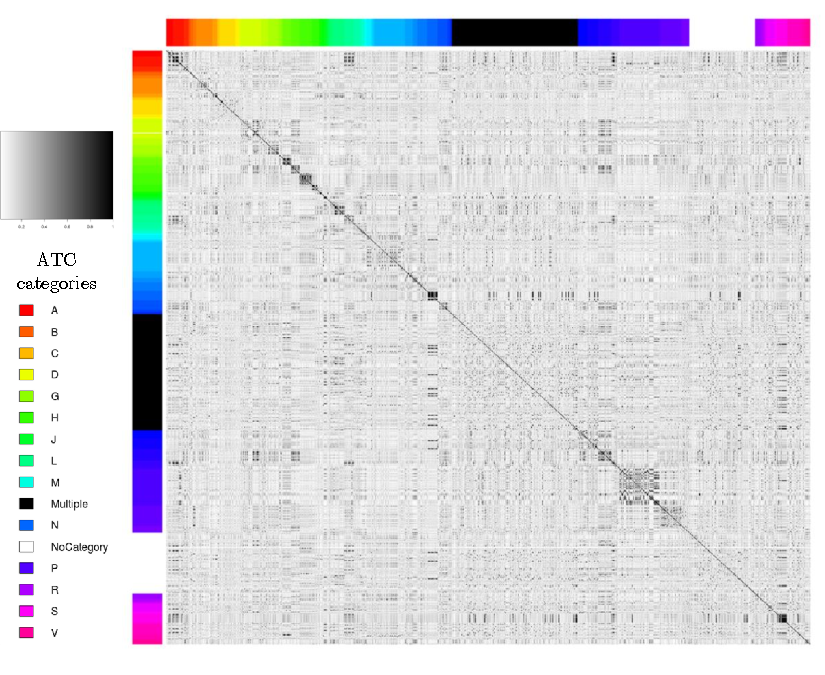
\includegraphics{fig3-13}
    \caption{Pairwise comparison of MoAs similarities. Therapeutic indications are represented by ATC categories which are the colours on the side. Two ATC level are considered on this graph, as opposite to picture 3-10, where only one level was considered. This increased resolution allows to identify more granular square patterns along the diagonal, where drugs from the same groups appear to have higher intensity values (no analyses performed).}
    \label{fig3-13}
\end{figure}

Figure 4 re-uses the same data as Figure \ref{fig3-14} (one ATC level) but with a clustering function apply to it (hierarchical clustering - manhattan distance) in order to reveal functional clusters of drugs (no analyses performed on this processing). Noteworthy, the taxonomic tree generated on the top of the data reflects the structure of the FTC.

\begin{figure}[H]
    \centering
    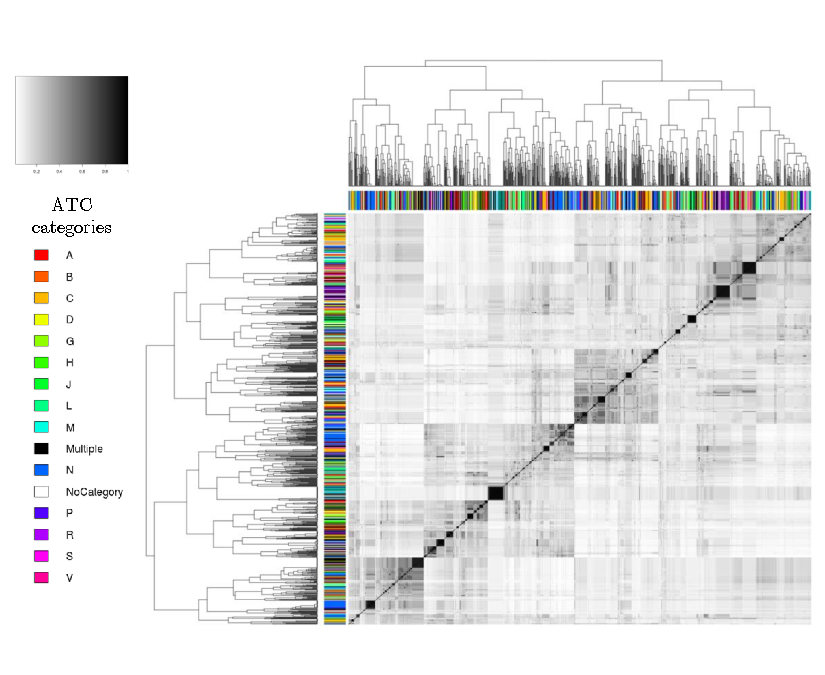
\includegraphics{fig3-14}
    \caption{Pairwise comparison of MoAs similarities. Therapeutic indications are represented by ATC categories which are the colours on the side. One ATC level is considered on this graph, just as picture \ref{fig3-12}. The similarity values are further clustered hierarchical clustering based on the Manhattan distance. This processing of the data enables to see functional clusters of drugs, namely groups of drugs with a similar pharmacology (no analyses presented in this document).}
    \label{fig3-14}
\end{figure}

Pairwise comparison of MoAs similarities. Therapeutic indications are represented by ATC categories which are the colours on the side. One ATC level is considered on this graph, just as picture \ref{fig3-12}. The similarity values are further clustered hierarchical clustering based on the Manhattan distance. This processing of the data enables to see functional clusters of drugs, namely groups of drugs with a similar pharmacology (no analyses presented in this document).

\begin{figure}[H]
    \centering
    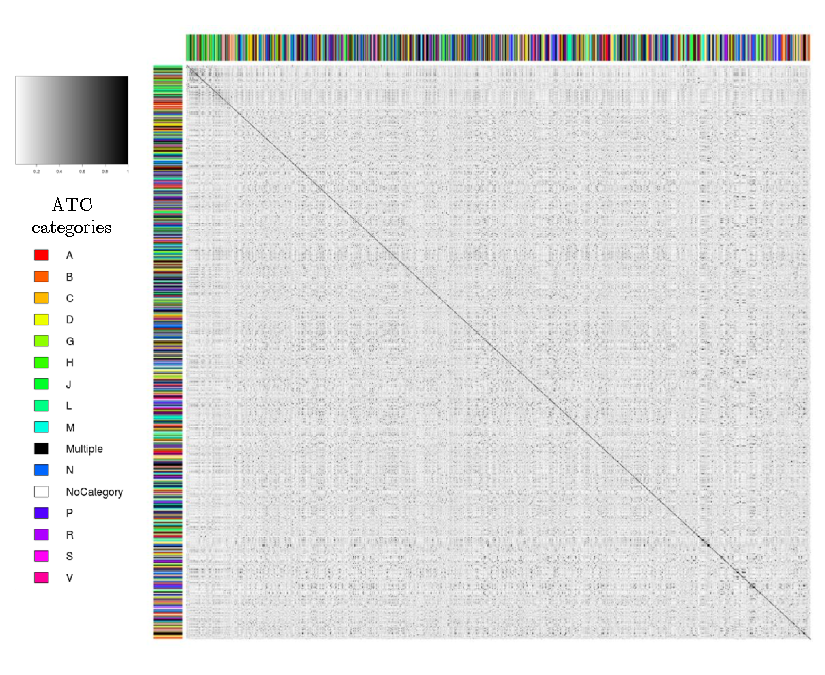
\includegraphics{fig3-15}
    \caption{Control pairwise comparison of MoAs similarities. Therapeutic indications are represented by ATC categories which are the colours on the side. One ATC level is considered on this graph, just as picture \ref{fig3-12}. Drugs are randomly sorted (yet symmetrically). No visual pattern is observable in this case, as opposed to what is seen on figures \ref{fig3-12}, \ref{fig3-13} and \ref{fig3-14}.}
    \label{fig3-15}
\end{figure}

Taken together, these results emphasise that the MoAs as defined in the FTC are indeed on average associated with the therapeutic indication of a drug. This result supports the validity of the resource and its potential to computationally address indication discovery. Further analyses are presented in Chapter 4, also integrating the concept of chemical structure.

\section{Discussion}
The FTC is a novel classification for approved drugs, which can be used as a starting point to generate drug repurposing hypotheses. This classification leverages the information present in various databases and ontologies, similarly to the Open PHACTS initiative \citep{williams2012open} and to the work done by \cite{hoehndorf2012identifying} and \citep{jupp2012logical}. The FTC mostly differentiates itself from these projects by providing a whole set of new categories on the top of the integrated information, dedicated to tackle a very specific problem: drug repositioning. Moreover, the semantic model behind the integration is richer than any of the previous approaches: FTC properties are expressive, thanks to the use extensive of transitive or chained property axioms (see section \ref{specskb}).

\subsection{Biological assumptions}
An asset of the FTC is its ability to handle efficiently categorical data: Classes and relationships are accurately defined, in order to classify compounds based on the semantics of their relations. The properties linking drugs to their respective protein targets (\emph{positive} and \emph{negative perturbations}) are however simplistic. At the time being, no consideration is given regarding the binding strength between the drug and the proteins, yet it is a key factor to derive potent and specific activities in the human body. This is also the case for other types of numerical data, such as the dosage; the FTC can predict a role for a drug, yet it cannot provide any information about the concentration or the administration route necessary to obtain the potential effects. The current relations between targets and their involvement in biological processes are also not a fully accurate representation of the biological phenomenon. In a cell, specific domains of the protein could mediate different functions. Only one of such activity types can sometimes be inhibited by a drug \citep{kruger2012mapping}, yet we are assuming in the FTC that as long as a drug affects a protein, it can therefore alter all its known functions. These limitations come from the semantics behind the axioms structuring the classification, themselves based on the information available from the databases. Despite entailing not entirely accurately the biochemical reality, the axioms help to generate a larger number of hypotheses, the primary goal of the FTC and inline with the theory presented on Chapter 2. The dosage issue is partially addressed by the \emph{regulator pattern} (see section \ref{catfunc}): It should be easier to experimentally adjust the concentration of the compounds classified as \emph{pro} or \emph{anti} biological process agents in order to modulate a physiological effect.

The predictions generated by the FTC depend on the resolution of the curated information released by the original data providers. Erroneous or missing information will lead to misclassification by the reasoner. Some expected outcomes are also missing from the predictions; \emph{sildenafil} for instance was expected to be classified as \emph{pro-penile erection agent} (FTC\_A0043084), yet the lack of appropriate GO annotation prevents it. After discussion with the GOA curation team, a manual annotation can only be asserted based on published experimental results. No document was found to support the involvement of the cGMP-specific 3',5'-cyclic phosphodiesterase (\emph{sildenafil}'s main target) in the \emph{negative regulation of penile erection} (GO:0060407), therefore no annotation can be made. Further work could be done in this direction, by trying to automatically infer more annotations or by using the electronically generated ones, in order to generate broader yet potentially less plausible repurposing hypotheses.

\subsection{Interpreting the evaluation}
Out of the evaluation, the high recall value (89\%) supports the idea behind the automated build of the FTC: The data from different repositories funded and curated in parallel, can be integrated to automatically create a new resource. This new classification (FTC) contains most of the known information present in an external gold standard (ATC) and relies on description logics to leverage the native information. In the context of this work I compared the content of the FTC against the ATC, knowing that these two taxonomies have diverging goals. During the evaluation, equivalences have been manually asserted between classes, which are assumed to have fairly similar meaning and containing similar sets of compounds. These manual assertions are however a weakness, as they are themselves not evaluated (free parameter). The presence or absence of a link was determined only by one curator and any mistake can influence consequently the recall and precision values. The precision of 50\% tells that the FTC tends to over-assigns compounds to MoA categories. The low precision value is acceptable in this case, as one of the underlying motivation of the FTC is to broadly represent polypharmacology, specially the one not present in gold standards such as the ATC, referencing only regulated usage. In this regard, the evaluation should be considered more as a safety control rather than a formal assessment of a predictive method.

The false positives derived from the evaluation can also be considered as drug repurposing hypotheses: These drugs can indeed be interpreted as suitable for the ATC category, yet not indexed as such. However, these predictions should be interpreted with caution, as it is currently impossible to distinguish a false positive from a reprofiling opportunity. These considerations do not interfere with the exploration based on semantic similarities. Finally, note that the ATC/FTC equivalences are open and editable online, any modification will be automatically incorporated in the next release of the resource. It is also possible to evaluate the FTC against a different taxonomy, like the Medical Subject Headings for example, which can be subject to future work.

\section{Summary}
The representation of the MoA as motivated in Chapter 1 was presented in this chapter. The axioms behind the resource and the deductions reached by the reasoner follow the theory introduced in Chapter 2. Despite the large size of the knowledge base, the classification process is fast and scalable, thanks to the EL++ profile. I will further present an analysis of the relationship between the MoA, the indication of a drug and its molecular structure in the coming chapter. Drug repositioning use-cases, not presented in the section, will also be discussed.

To conclude, the FTC is public resource, which can assist drug repositioning initiatives or enhance computational studies that evaluate drugs according to their \emph{mode of action}. The resource attributes biomolecular functions and processes to drugs, the same way as GO types have been assigned to gene products; its role is analogous to the one of a toolbox, classifying items based on their use (see Figure \ref{fig3-16}).

\begin{figure}[H]
    \centering
    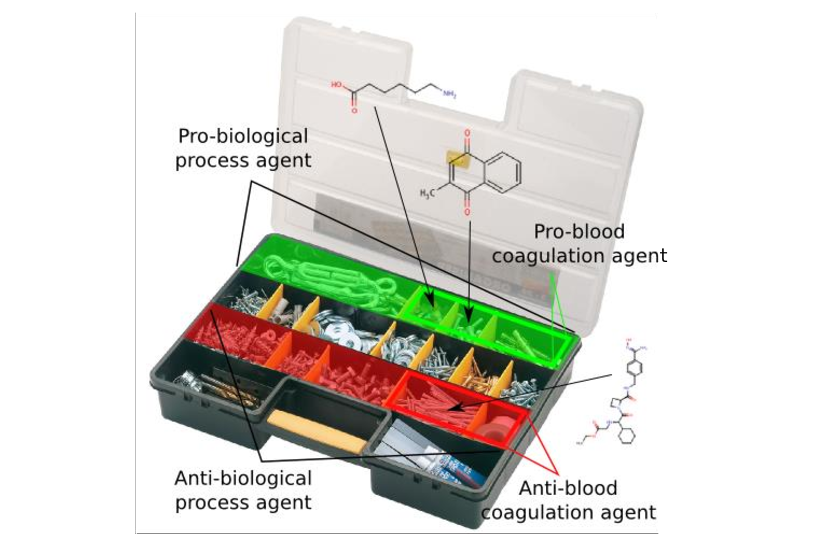
\includegraphics{fig3-16}
    \caption{Pharmacological toolbox analogy. The FTC describes categories inside which drugs can be classified; the classification helps to select the right tool for the right task, similarly to a toolbox.}
    \label{fig3-16}
\end{figure}

The construction of FTC relies on an axiomatic representation as the core means to attribute and derive the MoA for approved drugs. I showed the validity of the approach by comparing the content of the FTC to a well established clinical gold standard, the ATC. In Chapter 4, I analyse the FTC’s content to illustrate how repositioning hypotheses can be generated for hypertension treatment and Alzheimer's disease, using two different methodologies.

